% Correcting the title chapter page
\fancypagestyle{plain}{%
    \fancyhf{}
    \fancyhead[RO,LE]{\bfseries \thepage}
    \fancyhead[CO]{\rightmark}
    \fancyhead[CE]{\leftmark}
    \renewcommand{\headrulewidth}{0.4pt}}

\appendix

\cleardoublepage
\vspace*{8cm}
\thispagestyle{empty}
\begin{flushright}
\Huge \bfseries Dodaci
\end{flushright}
\cleardoublepage

\chapter{Kristalografske oznake i grupe}
\label{sec:kristalografija}
\textbf{Ireducibilne reprezentacije} $\Gamma^{(\alpha)}$ se obično označavaju
velikim slovima i to tako da se 1D reprezentacije označavaju slovima
$A$ i $B$, 2D reprezentacije slovom $E$, 3D reprezentacije slovom $T$
itd. Par kompleksno konjugiranih 1D reprezentacija se smatra jednom
2D reprezentacijom (jer ih povezuje vremenska inverzija) tako da se
one udružuju vitičastom zagradom i označavaju s $E$.

\textbf{Klase konjugacije} se obično označavaju simbolom $mC_n$ gdje je $m$
broj elemenata klase, a $C_n$ tipični predstavnik klase označen
Sch\"{o}nfliesovim simbolom:
\begin{center}
\begin{tabular}{rcp{10cm}}
$E$ & = & identiteta \\
$C_n$ & = & rotacija za $2\pi/n$ \\
$\sigma$ & = & refleksija preko ravnine \\
$\sigma_{h}$ & = & refleksija preko ``horizontalne'' ravnine tj. ravnine
  okomite na os najveće rotacijske simetrije \\
$\sigma_{v}$ & = & refleksija preko ``vertikalne'' ravnine tj. ravnine
  koja sadrži os najveće rotacijske simetrije \\
$\sigma_{d}$ & = & refleksija preko ``dijagonalne'' ravnine tj. ravnine
  koja sadrži os najveće rotacijske simetrije i raspolavlja kut između
  dvije $C_2$ osi okomite na tu os. (Specijalni slučaj $\sigma_{v}$.) \\
$S_n$  & = & rotacija za $2\pi/n$ kombinirana s refleksijom preko ravnine
   okomite na os te rotacije (Ove dvije operacije komutiraju.) \\
$i$ & = &  $S_2 \;\, = \;\,$  inverzija $\vec{r} \to -\vec{r}$
\end{tabular}
\end{center}
Ako ima više istovrsnih klasa, označavamo ih po redu npr.
$C_{2}$, $C_{2}'$, $C_{2}''$, itd.

\textbf{Točkaste grupe} kristala se označavaju slijedećim
Sch\"{o}nfliesovim oznakama:
\begin{center}
\begin{tabular}{rcl}
$C_n$ & = & grupe s jednom $C_n$ osi simetrije \\
$C_{nv}$ & = & grupe s jednom $C_n$ osi i $n$ $\sigma_v$
   refleksijskih ravnina  \\
$C_{nh}$ & = & $C_n$ os,  $\sigma_h$ refleksija $+$ dodaci \\
$S_{n}$ & = & $S_n$ os \\
$D_{n}$ & = & $C_n$ os i $n$ $C_2$ osi okomitih na nju \\
$D_{nd}$ & = & elementi od $D_{n}$ i $\sigma_d$ ravnine refleksije \\
$D_{nh}$ & = & elementi od $D_{n}$ i $\sigma_h$ ravnina refleksije \\
$T$  & = & tetrahedralna grupa \\
$O$  & = & oktahedralna grupa 
\end{tabular}
\end{center}

\textbf{Tablice karaktera} nekih grupa koje se pojavljuju u ovoj knjizi

Ciklička grupa C$_3$:
\begin{center}
\begin{tabular}{c|ccc}
     & $E$ & $C_3$ & $C_{3}^2$ \\ \hline
    $A$ & 1 & 1 & 1 \\
    \multirow{2}{*}{$E$} & 1 & $\omega$ & $\omega^2$ \\
     & 1 & $\omega^2$ & $\omega$ \\
\end{tabular}
\end{center}
gdje je $\omega = e^{2\pi i/3}$ kubni korijen jedinice i
gdje su zadnje dvije ireducibilne reprezentacija međusobno
kompleksno konjugirane pa se često smatraju jednom dvodimenzionalnom
reprezentacijom $E$.

Ciklička grupa C$_4$:
\begin{center}
\begin{tabular}{c|cccc}
     & $E$ & $C_4$ & $C_2$ & $C_{4}^3$ \\ \hline
    $A$ & 1 & 1 & 1 & 1 \\
    $B$ & 1 & -1 & 1 & -1 \\
    \multirow{2}{*}{$E$} & 1 & $i$ & -1 & $-i$ \\
     & 1 & $-i$ & -1 & $i$ \\
\end{tabular}
\end{center}

Kleinova četvorna grupa D$_2$
\begin{center}
\begin{tabular}{c|cccc}
     & $E$ & $C_{2}(z)$ & $C_{2}(y)$ & $C_{2}(x)$ \\ \hline
    $A_1$ & 1 & 1 & 1 & 1 \\
    $B_1$ & 1 & 1 & -1 & -1 \\
    $B_2$ & 1 & -1 & 1 & -1 \\
    $B_3$ & 1 & -1 & -1 & 1 \\
\end{tabular}
\end{center}

Dihedralna grupa D$_3$
\begin{center}
\begin{tabular}{c|ccc}
  & E & 2$C_3$  & 3$C_2$ \\ \hline
$A_1$ & 1 & 1& 1 \\
$A_2$ & 1 & 1&-1 \\
 $E$  & 2 &-1& 0
\end{tabular}
\end{center}


Dihedralna grupa D$_{4}$
\begin{center}
    \begin{tabular}{c|ccccc}
         & $E$ & $2C_4$ & $C_2$ & $2C_{2}'$ & $2C_{2}''$ \\ \hline
        $A_1$ & 1 & 1 & 1 & 1 & 1 \\
        $A_2$ & 1 & 1 & 1 & -1 & -1 \\
        $B_1$ & 1 & -1 & 1 & 1 & -1 \\
        $B_2$ & 1 & -1 & 1 & -1 & 1 \\
        $E$ & 2 & 0 & -2 & 0 & 0 \\
    \end{tabular}
\end{center}
Ova je grupa izomorfna grupi C$_{4v}$, samo što su u tom  slučaju
neke rotacije za $\pi$ zapravo refleksije: $C_{2}' \to \sigma_v$ i
$C_{2}'' \to \sigma_h$.


Tetrahedralna grupa T:

\begin{center}
\begin{tabular}{c|cccccccc}
 & $E$ & $3C_2$ & $4C_3$ & $4C_{3}^2$  \\ \hline
$A$ & 1 & 1 & 1 & 1  \\
\multirow{2}{*}{$E$} & 1 & 1 & $\omega$ & $\omega^2$ \\
 & 1 & 1 & $\omega^2$ & $\omega$  \\
$T$ & 3 & -1 & 0 & 0  \\
\end{tabular}
\end{center}
gdje je $\omega = e^{2\pi i/3}$ kubni korijen jedinice.



\chapter{Aksijalni vektori (pseudovektori)}
\label{sec:aksijalni}

\emph{Aksijalni} ili \emph{pseudovektori} su objekti koji se pri rotacijama transformiraju
isto kao i obični (tzv. \emph{polarni}) vektori, ali pri refleksijama i inverzijama
imaju još i dodatnu promjenu predznaka.

Inverzija običnim vektorima u 3D euklidskom prostoru mijenja
predznak 
$$i: \vec{r} \to - \vec{r}$$ 
i može se reprezentirati dijagonalnom
matricom 
$$
i = -\Eins = 
\begin{pmatrix}
    -1 & 0 & 0 \\
    0 & -1 & 0 \\
    0 & 0 & -1
\end{pmatrix} \;.
$$
No, vektorski produkt dvaju polarnih vektora, npr. vektora položaja $\vec{r}$
i impulsa $\vec{p}$ posljedično \emph{ne mijenja} predznak:

\[  \vec{L}\equiv \vec{r}\times\vec{p} \; \stackrel{i}{\longrightarrow} \;
  (-\vec{r}) \times (-\vec{p}) =  \vec{r}\times\vec{p} = \vec{L}  \;,
\]

što znači da je $\vec{L}$ (moment impulsa) aksijalni vektor. (U fizici su
veličine vezane uz vrtnju, poput momenta impulsa ili momenta sile, 
često reprezentirane aksijalnim vektorima. Isto vrijedi za veličine
vezane uz magnetizam koji je obično rezultat kruženja (mikro ili makro) struja.)

Da bi se naglasila njihova različitost,
ponegdje u literaturi se aksijalne vektore ne crta kao usmjerene crte
(strelice), već kao crte s ``aksijalnim strelicama'' (cf. 
\cite{Bronstejn:2004} p. 186)

\centerline{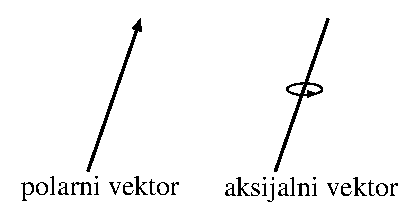
\includegraphics[scale=0.8]{pics/aksijalni_vektor.eps}}

Slično definiramo \emph{pseudoskalarne} veličine kao one koje su skalari
obzirom na rotacije, ali mijenjaju predznak pri refleksijama i inverzijama.
Npr. miješani produkt polarnih vektora je pseudoskalar:

\[
P = (\vec{r}_1 \times \vec{p}) \cdot \vec{r}_2  \; \stackrel{i}{\longrightarrow} \;
  - (\vec{r}_1 \times \vec{p}) \cdot \vec{r}_2 = - P
\]

Magnetski moment, definiran kao $\vec{M} = \frac{1}{2} \int \vec{r}
\times \vec{J} dV$ za gustoću struje $J$, odnosno kao
$\vec{M} = \frac{1}{2} q \vec{r} \times \vec{v}$ za točkasti
naboj $q$, je dakle aksijalni vektor.

Ovaj koncept se generalizira i na tenzore odnosno pseudotenzore višeg ranga.
Važan je primjer Levi-Civita pseudotenzor trećeg ranga koji je invarijantan
pri rotacijama, ali mijenja predznak pri refleksijama, u što se možemo uvjeriti
korištenjem njegovog svojstva iz zadatka \ref{zad:levicivita} i svojstva
determinanti elemenata O(3) grupe sa stranice \pageref{pag:detO3}.

Za još o pseudovektorima i drugim pseudo-veličinama vidi
npr. \cite{Arfken:1995}.


\chapter{Kvantna mehanika u Diracovoj notaciji}
\label{sec:qm}

\textbf{Fizikalno stanje} kvantnomehaničkog sustava
je reprezentirano vektorom u Hilbertovom prostoru za
koji se koristi Diracova oznaka
 $\ket{\alpha}$ --- tzv. "ket". 
(Strogo uzevši, kvantnom stanju odgovara
čitava "zraka" $c\ket{\alpha}, c\in\mathbb{C}$.)

Simbol $\alpha$ ovdje stoji za sve kvantne brojeve koji su potrebni za potpuno
određenje stanja. Npr, za vodikov atom $\ket{\alpha}=\ket{n,l,m}$.
Svakom vektoru odgovara dualni "bra" vektor $\bra{\alpha}$, tako
da skalarni produkt zapisujemo kao "bra-ket"A
$\bra{\alpha}\beta \rangle$. Kako je riječ o vektorskom prostoru
nad kompleksnim poljem, vrijedi
$\bra{\alpha}\beta \rangle^{*} = \bra{\beta}\alpha \rangle$.

\textbf{Opservabla} (veličina koja se eksperimentalno određuje i ima
 analogon u klasičnoj fizici) je reprezentirana hermitskim operatorom na
 Hilbertovom prostoru prostoru stanja: $A=A^{\dagger}$.

Ako su $\ket{a}$ svojstveni vektori od $A$ sa svojstvenim vrijednostima
$a$, tj.
\begin{displaymath}
                A\ket{a}=a\ket{a} \;,
\end{displaymath}
onda mjerenje klasične veličine koja odgovara operatoru A, na sustavu
opisanom vektorom $\ket{\alpha}$, s vjerojatnošću $|\bra{a}\alpha\rangle|^2$
ima ishod $a$, nakon čega sustav "skače" u stanje $\ket{a}$.

Očekivana vrijednost mjerenja veličine koja odgovara
operatoru $A$, na sustavu opisanom vektorom stanja
$\ket{\alpha}$ je $\bra{\alpha}A\ket{\alpha}$.

Svi svojstveni vektori nekog hermitskog operatora čine jednu bazu
Hilbertovog prostora:
\begin{displaymath}
             \sum_{a} \ket{a}\bra{a} = 1 \,.
\end{displaymath}
Npr. svi vektori $\ket{\vec{r}}$ čine jednu tzv. koordinatnu bazu.
Schr\"{o}dingerova valna funkcija $\psi_{\alpha}(\vec{r})$ su zapravo
komponente vektora stanja $\ket{\alpha}$ prikazane u koordinatnoj
bazi:
\begin{displaymath}
            \psi_{\alpha}(\vec{r})=\bra{\vec{r}}\alpha\rangle
\end{displaymath}


\textbf{Operatori transformacije} fizikalnog sustava (tj. odgovarajućeg vektora
stanja) moraju biti unitarni i linearni (ili antiunitarni i antilinearni)
\begin{align*}
\text{\sl unitarnost}&:\; \bra{U\alpha}U\beta\rangle = \bra{\alpha}\beta\rangle
   \\
\text{\sl linearnost}&:\; U\big(c_1\ket{\alpha}+c_{2}\ket{\beta}\big)=
  c_1 U\ket{\alpha} + c_{2} U\ket{\beta}
   \\[2ex]
\text{\sl antiunitarnost}&:\; \bra{U\alpha}U\beta\rangle = \bra{\alpha}\beta\rangle^*
  \\
\text{\sl antilinearnost}&:\; U\big(c_1\ket{\alpha}+c_{2}\ket{\beta}\big)=
  c_{1}^* U\ket{\alpha} + c_{2}^* U\ket{\beta}
\end{align*}
Ovo je sadržaj tzv. Wignerovog teorema, a u osnovi
je posljedica zahtjeva za očuvanjem vjerojatnosti i
načela superpozicije u kvantnoj mehanici.

Za korektan matematički opis kvantne mehanike, stanja u Hilbertovom
prostoru nisu dovoljna. Na primjer, svojstvena stanja važnih operatora
impulsa, $e^{i p x}$, i položaja, $\delta(x - x_0)$, \emph{nisu} elementi
Hilbertovog prostora. Prvi jer mu je norma beskonačna, a drugi jer mu
norma nije ni definirana (norma je $\int \rmd x \psi^{*}(x) \psi(x)$,
a kvadrat Diracove delta funkcije nije definiran).
Stoga se Hilbertov prostor stanja treba upotpuniti tzv. generaliziranim
funkcijama poznatim i kao \emph{distribucije}. Distribucije nisu nužno
definirane svojom vrijednosti u pojedinim točkama nego samo kao funkcionali
tj. preslikavanja s prostora funkcija na polje kompleksnih brojeva $\mathbb{C}$.
Klasičan primjer distribucije je Diracova delta funkcija $\delta_{x_0}$ koja je definirana
kao preslikavanje koje nekoj pitomoj (tzv. \emph{testnoj}) funkciji $f(x)$
pridružuje broj $\delta_{x_0}(f) = f(x_0)$. Sve "obične" funkcije $g(x)$ su isto
i distribucije gdje je preslikavanje standardni integral  $\int \rmd x g^{*}(x) f(x)$,
pa se često takvim integralom formalno zapisuje i djelovanje distribucije
$\int \rmd x \delta(x-x_0) f(x) = f(x_0)$, ali to je samo formalni zapis
koji ne odgovara matematičkoj integraciji u smislu Riemanna ili Lebesguea.
Prostor $\Phi$ testnih funkcija  na koje distribucije mogu smisleno djelovati je
manji od Hilbertovog (tipično se uzima prostor tzv. Schwartzovih funkcija koje su glatke
i imaju svojstvo da one same i sve njihove derivacije padaju u beskonačnosti brže od svake potencije),
dok je prostor
distribucija $\Phi^{\times}$ kako smo vidjeli veći od Hilbertovog.
Cijela ta trojka
\begin{equation}
    \Phi \subseteq \mathcal{H} \subseteq \Phi^{\times} \;,
    \label{eq:gelfand}
\end{equation}
naziva se \emph{opremljeni} (\emph{rigged}) Hilbertov prostor  ili
\emph{Gel'fandov triplet} \cite{Ballentine:1998}. Tako, sasvim strogo uzevši, Diracovi
"ket" simboli predstavljaju elemente ovog najvećeg prostora $\Phi^{\times}$.
Srećom, ove matematičke finese često nisu ključne i
manipulacije vektorima kao u konačnodimenzionalnim vektorskim prostorima i distribucijama
kao običnim funkcijama u velikom broju slučajeva vode na ispravne rezultate.



\chapter{Tenzori kao matematički strojevi}
\label{sec:tenzorKaoStroj}

Tenzore možemo promatrati kao neku vrstu \emph{matematičkih strojeva}
\cite{MTW:2017}
čiji "input" su jedan ili više vektora, a "output" vektor ili
skalar. 

Praktično, problemi kojima se bavimo se gotovo uvijek daju formulirati
u obliku "\emph{Znamo te i te vektore koji opisuju sustav. Koliki
je $s$ ili $\vec{v}$ tog sustava?}", gdje su $s$ i $\vec{v}$ neki
zanimljivi skalari ili vektori (energija, impuls, položaj, \dots).

Označimo tip tenzora $\bbtensor{T}$ s uređenim parom $(0, n)$ ukoliko 
$\bbtensor{T}$ predstavlja stroj čiji input je $n$ vektora, a output skalar,
a s $(1, n)$ ukoliko je output vektor. Takav stroj
možemo skicirati kao
\begin{equation}
   \bbtensor{T}(\underbrace{\slot, \slot, \slot, \dots}_{n \times})  \;,
\end{equation}

gdje su ``$\rule{1em}{1pt}$'' mjesta gdje treba staviti konkretne vektore
koje će onda stroj ``preraditi'' u rezultirajući skalar ili vektor

\begin{equation}
   \bbtensor{T}(\vec{v}_1, \vec{v}_2, \dots) = s \quad \text{ili} \quad \vec{v} \;.
\end{equation}

Na primjer, klasični vektor \emph{sile} možemo interpretirati kao
$(0, 1)$ tenzor $\bbtensor{SILA}(\slot)$ sa svojstvom da kad mu
u njegov slot stavimo vektor brzine dobijemo skalar snage:
\begin{equation}
   \bbtensor{SILA}(\vec{v}) = P
\end{equation}
gdje je unutranji ``mehanizam'' stroja dan jednadžbom $P = \vec{F}\cdot\vec{v}$.

Primjer $(0,2)$ tenzora je metrički tenzor $\bbtensor{G}(\slot, \slot)$,
čiji je mehanizam takav da kad u njegove slotove stavimo dva vektora
dobijemo njihov skalarni produkt:

\begin{equation}
   \bbtensor{G}(\vec{a}, \vec{b}) = \vec{a}\cdot\vec{b} \;.
\end{equation}

Ono što se često naziva tenzorom drugog ranga (matrica brojeva) su
samo komponente tenzora u nekoj bazi, koje se
dobiju kad se pravom apstraktnom tenzoru u njegove input slotove
stave jedinični bazni vektori, npr,

\begin{equation}
   \bbtensor{G}(\vec{e}_i, \vec{e}_j) = g_{ij} \;.
\label{eq:Gkomponente}
\end{equation}

Tenzor gustoće vodljivosti iz prošlog odjeljka je dakle
tipa $(1,1)$, odnosno $\sigma(\slot)$, jer imamo
$\sigma(\vec{E}) = \vec{j}$, dakle jedan vektor kao input
i drugi kao output.

Totalno antisimetrični tenzor (Levi-Civita) u tri dimenzije je
tenzor oblika $(1, 2)$, u svom obliku u kojem nam daje
vektorski produkt dvaju vektora
\begin{equation}
   \bbtensor{LEVICIVITA}(\vec{a}, \vec{b}) = \vec{a}\times\vec{b} \;,
\end{equation}
ali on može biti u obliku $(0, 3)$ kad daje mješani produkt 
triju vektora
\begin{equation}
   \bbtensor{LEVICIVITA}'(\vec{a}, \vec{b}, \vec{c}) =
 (\vec{a}\times\vec{b})\cdot\vec{c} \;,
\end{equation}
gdje ta dva oblika nisu identična.

U elektrodinamici (koja je teorija koja poštuje specijalnu teoriju
relativnosti), javlja se $(1,1)$ tenzor $\bbtensor{FARADAY}$, ali koji
nije tenzor obzirom na rotacije
već obzirom na relativističke transformacije u četverodimenzionalnom
prostoru Minkowskog. Taj tenzor daje četverovektor Lorentzove sile
kad mu se kao input stavi četverovektor brzine
$\bbtensor{FARADAY}(\vec{u)} = F_{\rm Lorentz}$, odnosno u uobičajenom
zapisu po komponentama $\mu, \nu = 0,1,2,3$, 
$F^{\mu}_{\rm Lorentz} = d p^{\mu}/d\tau = e F^{\mu}_{\,\nu} u^\nu$.

\secret{
Riemannov tenzor zakrivljenosti plohe spomenut u prošlom odjeljku 
je $(1, 3)$ tenzor
koji kad dobije vektore brzine dvaju čestica i njihove udaljenost,
daje ubrzanje kojim se one približavaju ili udaljavaju na toj plohi.}

\subsubsection*{Apstraktna indeksna notacija}

Indeksi na tenzorima najčešće označavaju kompenente tog tenzora
u nekoj bazi, vidi (\ref{eq:Gkomponente}). Međutim, moguće ih
je upotrebljavati i samo kao zamjenu za ove slotove koji su
nespretni za zapisivanje.

Tako npr.  za $(0, n)$ tenzor imamo korespondenciju
\begin{equation}
\bbtensor{T}(\slot,\slot,\slot, \dots)  \longrightarrow T_{abc\dots} \;,
\end{equation}
gdje se vektori onda zapisuju kao $V^a$ i npr.  $T_{ab}V^{a}V^{b}$ je
broj (skalar) dobiven ``kontrakcijom'' tenzora drugog ranga sa
dva vektora, uz konvenciju da se kontrakcija uvijek radi s jednim
gornjim i jednim donjim indeksom. Tenzor $(1,n)$ tipa bi onda bio
$T^{a}_{bcd\dots}$, a vektor $V^a$ je tenzor $(1,0)$ tipa (input
je ništa ili broj, a output je vektor).

Promotrimo sada objekt  $\bbtensor{G}(\vec{V},\slot)$, tj, metrički
tenzor s popunjenim jednim slotom, tj. $g_{ab}V^a$. Očito je da
taj objekt, ako ga kontrahiramo s još jednim vektorom $W^{b}$, daje skalar.
Dakle riječ je o tenzoru tipa $(0, 1)$, kojeg stoga možemo skraćeno
zapisati kao $V_a$.

Dakle tek taj objekt $V_a$, koji nije isto što i $V^a$, se može
skalarno množiti s vektorima da bi se dobio skalar. To što u praksi
u trodimenzionalnom vektorskom prostoru množimo skalarno vektore
međusobno je samo zato što je u tom prostoru metrički tenzor
jednak jediničnom 
\begin{displaymath}
g = \text{diag}(1, 1, 1) =
\begin{pmatrix}
1 & 0 & 0 \\ 0 & 1 & 0 \\ 0 & 0 & 1
\end{pmatrix}
\end{displaymath}
pa je \emph{po komponentama} $V^a$ jednak $V_a$.

U četverodimenzionalnom prostoru Minkowskog 
$g = \text{diag}(1, -1, -1, -1)$ pa $V^a$ i $V_a$ više nisu
ista stvar, ali to ne moramo jako naglašavati; dovoljno je
pri skalarnom množenju paziti na predznake:
$g_{\mu \nu} a^{\mu} a^{\nu} = a_{\mu} a^{\mu} = (a^{0})^2 
- \vec{a}\cdot\vec{a}$.

No, u općenitom zakrivljenom prostoru s općenitim metričkim
tenzorom moramo strogo razlikovati vektor $V^a$ i objekt
$V_a$ (za kojeg postoji i specijalno ime: \emph{1-forma}).
Npr. u Hilbertovom prostoru Diracov ``ket'' $|\alpha\rangle$ je
vektor, a ``bra'' $\langle\alpha|$ je 1-forma. Više o ovome
vidi u knjigama iz diferencijalne geometrije.

\chapter{Homomorfizam grupa \SU{2} i \SO{3}}
\label{sec:su2so3}

Kompletan dokaz 2-na-1 homomorfnosti \SU{2} i \SO{3} provest ćemo
u četiri koraka:
\begin{enumerate}
    \item Konstruirat ćemo preslikavanje iz \SU{2} u grupu svih invertibilnih realnih
        $3\times 3$ matrica $\GL{3, \mathbb{R}}$ i pokazati da je to preslikavanje homomorfizam.
    \item Pokazat ćemo da je slika preslikavanja sadržana u $\SO{3} \in \GL{3, \mathbb{R}}$.
    \item Pokazat ćemo da je preslikavanje surjekcija.
    \item Pokazat ćemo da se matrice U i -U iz \SU{2}, obje i samo one, preslikavaju u 
        istu matricu iz \SO{3}.
\end{enumerate}
Preliminarno, uočimo da se svaka $2\times 2$ matrica $M$ može zapisati kao linearna
kombinacija,
\begin{equation}
M = \alpha_0 \mathbb{I} + \alpha_i \sigma_i, \quad \alpha_0, \alpha_i \in \mathbb{C}\;,
\end{equation}
jedinične $\mathbb{I}$ i Paulijevih matrica
\begin{equation}
\sigma_1 = \begin{pmatrix} 0 & 1 \\ 1 & 0 \end{pmatrix}, \quad
\sigma_2 = \begin{pmatrix} 0 & -i \\ i & 0 \end{pmatrix}, \quad
\sigma_3 = \begin{pmatrix} 1 & 0 \\ 0 & -1 \end{pmatrix}\,,
\label{eq:paulijevematrice}
\end{equation}
jer je riječ o četiri linearno nezavisne matrice, koliko ima i elemenata $M$.
Ukoliko je $\mathrm{Tr} M = 0$,
onda je $\alpha_0 = 0$, a ukoliko je $M$ hermitska $\alpha_i$ su realni
(uvjerite se u ovo!).

\emph{1. korak.} Promotrimo matrice
\begin{equation}
    S_{i} = U \sigma_i U^\dagger \,,
\end{equation}
gdje je $U$ data matrica iz \SU{2}, a $\sigma_i$ su Paulijeve.
Zahvaljujući cikličnosti traga i unitarnosti $U^\dagger U = 1$ odmah vidimo da je
$\Tr S_i = 0$. Isto tako, zahvaljujući hermitičnosti Paulijevih
matrica imamo
\begin{equation}
    S_{i}^{\dagger} = (U \sigma_i U^\dagger)^\dagger = U \sigma_{i}^\dagger U^\dagger
    = S_{i} \,,
\end{equation}
dakle $S_{i}$ je i hermitična pa se može prikazati kao linearna kombinacija
Paulijevih matrica s realnim koeficijentima, $S_{i} = R_{ji}(U) \sigma_j$,
gdje smo naznačili da koeficijenti ovise o $U$. Tako imamo
\begin{equation}
    U \sigma_i U^\dagger = R_{ji}(U) \sigma_j \,,
    \label{eq:defRimp}
\end{equation}
što smatramo implicitnom definicijom $3 \times 3$ realne matrice $R$ i time smo konstruirali
preslikavanje sa \SU{2} na $\GL{3, \mathbb{R}}$. (Strogo uzevši, trebalo bi još pokazati da je $R$
regularna tj. $\det R \neq 0$, a to ćemo malo niže u drugom koraku dokaza.)
Množenjem ove jednadžbe sa $\sigma_{k}$ s desne strane, uzimanjem traga i korištenjem
$\Tr \sigma_{j}\sigma_{k} = 2\delta_{jk}$ (vidi zadatak \ref{zad:svojstvapaulijevih})
dobivamo eksplicitnu definiciju matrice $R$:
\begin{equation}
    R_{ij}(U) = \frac{1}{2} \Tr\left(\sigma_i U \sigma_j U^\dagger \right).
    \label{eq:defReksp}
\end{equation}
Sada treba pokazati da je ovakvo preslikavanje homomorfizam.
Za bilo koje $U, V \in SU(2)$ vrijedi
\begin{align}
    R_{ij}(UV)& = \frac{1}{2} \Tr\left( \sigma_i (UV) \sigma_j (UV)^\dagger \right) \\
              & = \frac{1}{2} \Tr\left(\sigma_i U \left(V  \sigma_j V^\dagger\right) U^\dagger\right) \\
              & = R_{kj}(V)\frac{1}{2} \Tr\left(\sigma_i U \sigma_k U^\dagger \right) \\
              & = R_{kj}(V) R_{ik}(U) \\
              & = \big(R(U) R(V) \big)_{ij}\,,
\end{align}
gdje smo između ostalog koristili linearnost traga. Time smo pokazali
da je preslikavanje homomorfno.


\emph{2. korak.} 
Razmotrimo produkt \( U \sigma_i \sigma_j U^\dagger \).  S jedne strane prvo
možemo raspisati produkt Paulijevih matrica pa onda primijeniti (\ref{eq:defRimp}) 
\begin{align}
    U \sigma_i \sigma_j U^\dagger& =  U \left(
        \delta_{ij} \mathbb{I} + i \epsilon_{ijk}\sigma_{k} \right) U^\dagger \\
                                 & = \delta_{ij} \mathbb{I} + i \epsilon_{ijk}
                                 R_{nk} \sigma_n \,.
                                 \label{eq:tautau1}
\end{align}
S druge strane, možemo prvo ubaciti $U^\dagger U = 1$ između dvije Paulijeve
matrice i dvaput primijeniti (\ref{eq:defRimp}) pa tek onda rastaviti produkt
Paulijevih matrica
\begin{align}
    U \sigma_i \sigma_j U^\dagger& =  U \sigma_i U^\dagger U \sigma_j U^\dagger \\
                                 & = R_{li} \sigma_{l} R_{mj} \sigma_{m} \\
                                 & = R_{li} R_{mj} \left(
        \delta_{lm} \mathbb{I} + i \epsilon_{lmn}\sigma_{n} \right) \\
                                 & = (R^{\mathsf{T}} R)_{ij} \mathbb{I}
                     + i R_{li} R_{mj}\epsilon_{lmn}\sigma_{n} \,.
                                 \label{eq:tautau2}
\end{align}
Usporedbom koeficijenata ispred jediničnih matrica vidimo da je
$(R^{\mathsf{T}} R)_{ij} = \delta_{ij}$ čime smo pokazali da je $R$ ortogonalna.
Treba još pokazati da je njena determinanta 1. Izjednačavanjem
koeficijenata u (\ref{eq:tautau2})  i (\ref{eq:tautau1}) uz Paulijeve matrice
i množenjem s $R_{ns}$ imamo
\begin{equation}
    R_{li} R_{mj}R_{ns}\epsilon_{lmn} = \epsilon_{ijk} \underbrace{R_{nk} R_{ns}}_{=\delta_{ks}}
    = \epsilon_{ijs}
\end{equation}
S druge strane, koristeći svojstva Levi-Civita tenzora (vidi zadatak \ref{zad:svojstvalevicivite})
imamo
\begin{align}
 \det R& = \frac{1}{3!} R_{li} R_{mj}R_{ns} \epsilon_{lmn} \epsilon_{ijs}  \\
       & = \frac{1}{3!} \epsilon_{ijs}\epsilon_{ijs} = 1\,.
\end{align}
Ovo je dobra vježba iz manipulacija Levi-Civita tenzorom, ali postoji i jednostavniji
način da se vidi da je $\det R = 1$. 
Po svojstvu homomorfizma, jedinični element iz \SU{2} se preslikava u jedinični
element iz \SO{3}, koji ima determinantu 1.
Nadalje, grupna mnogostrukost od \SU{2} je takva da se
svaki element može doseći od jediničnog kontinuiranim gibanjem po grupnoj mnogostrukosti
(kažemo da je ona \emph{povezana}, vidi kasnije definiciju \ref{def:povezanost}).
No i preslikavanje (\ref{eq:defReksp}) je kontinuirano i tim kontinuiranim gibanjem
po \SU{2} se $\det R$ ne može diskontinuirano promijeniti s +1 na -1, što znači da je slika
preslikavanja upravo \SO{3}.

\emph{3. korak.} 
Pokazat ćemo da se svaka rotacija može prikazati kao (\ref{eq:defRimp}) 
tako da eksplicitno konstruiramo odgovarajuću matricu $U \in \SU{2}$.
Kao prvo, podsjetimo se činjenice da se proizvoljna rotacija može prikazati
kao kompozicija rotacija oko $z$-osi, $y$-osi, pa opet $z$-osi za tri,
tzv. Eulerova kuta (vidi npr. \cite{Sakurai:2011})
\begin{equation}
R = R_{3}(\gamma) R_{2}(\beta) R_{3}(\alpha) \,.
\end{equation}
Rotaciji $R_{3}(\alpha)$  oko $z$-osi
\begin{equation}
   R_{3}(\alpha) = 
   \begin{pmatrix}
       \cos\alpha & \sin\alpha & 0 \\
      -\sin\alpha & \cos\alpha & 0 \\
       0 & 0 & 1
   \end{pmatrix}
\end{equation}
odgovara element
\begin{equation}
    U_{3}(\alpha) =   \cos\frac{\alpha}{2} + i \sigma_{3} \sin\frac{\alpha}{2} =
    \begin{pmatrix}
        e^{i\alpha/2} & 0 \\
        0 & e^{-i\alpha/2}
    \end{pmatrix} \in \SU{2} \;.
\end{equation}
Provjeriti da je to tako možemo eksplicitnim raspisivanjem definicione
jednadžbe (\ref{eq:defRimp}) 
\begin{equation}
    U_{3}(\alpha) \sigma_i U_{3}(\alpha)^\dagger =
    R_{3}(\alpha)_{ji} \sigma_{j} = \big(R_{3}(\alpha)\big)^{\mathsf{T}}_{ij} \sigma_j \;.
\end{equation}
Po komponentama to je
\begin{align}
    U_{3}(\alpha) \sigma_1 U_{3}(\alpha)^\dagger& = \sigma_1 \cos\alpha - \sigma_2 \sin\alpha \\
    U_{3}(\alpha) \sigma_2 U_{3}(\alpha)^\dagger& = \sigma_1 \sin\alpha + \sigma_2 \cos\alpha \\
    U_{3}(\alpha) \sigma_3 U_{3}(\alpha)^\dagger& = \sigma_3
.\end{align}
Prvu od tih jednadžbi provjerimo raspisivanjem lijeve strane
\begin{align}
    U_{3}(\alpha) \sigma_1 U_{3}(\alpha)^\dagger & =
    \big(\cos\frac{\alpha}{2} + i \sigma_{3} \sin\frac{\alpha}{2}\big) \sigma_1
    \big(\cos\frac{\alpha}{2} - i \sigma_{3} \sin\frac{\alpha}{2}\big) \\
& =   \big(\sigma_1 \cos\frac{\alpha}{2} - \sigma_{2} \sin\frac{\alpha}{2})\big)
    \big(\cos\frac{\alpha}{2} - i \sigma_{3} \sin\frac{\alpha}{2}\big) \\
& =   \sigma_1 \big(\cos^{2}\frac{\alpha}{2} -  \sin^{2}\frac{\alpha}{2}\big)
  -   2 \sigma_2 \sin^{2}\frac{\alpha}{2}\cos^{2}\frac{\alpha}{2} \\
& =   \sigma_1 \cos\alpha -  \sigma_2 \sin\alpha \,.
\end{align}
Ostale dvije jednadžbe provjerimo na isti način, a istim postupkom možemo
vidjeti da se
\begin{equation}
    U_{2}(\beta) =   \cos\frac{\beta}{2} + i \sigma_{2} \sin\frac{\beta}{2} =
    \begin{pmatrix}
        \cos{\beta}/{2} & \sin{\beta}/{2} \\
        -\sin{\beta}/{2} & \cos{\beta}/{2}
    \end{pmatrix} \in \SU{2} \;,
\end{equation}
preslikava u
$R_{2}(\beta)$ rotaciju oko $y$-osi. Tako za proizvoljnu rotaciju imamo
\begin{equation}
U = 
    \begin{pmatrix}
        e^{i\gamma/2} & 0 \\
        0 & e^{-i\gamma/2}
    \end{pmatrix} 
    \begin{pmatrix}
        \cos{\beta}/{2} & \sin{\beta}/{2} \\
        -\sin{\beta}/{2} & \cos{\beta}/{2}
    \end{pmatrix}
    \begin{pmatrix}
        e^{i\alpha/2} & 0 \\
        0 & e^{-i\alpha/2}
    \end{pmatrix}  \in \SU{2}
\end{equation}
koji se u tu rotaciju preslikava, čime smo dokazali surjekciju.
Valja uočiti da su kutovi u \SU{2} polovice odgovarajućih kutova rotacija iz \SO{3},
što znači da period od $U$ nije $2\pi$ nego $4\pi$ što se, kako je diskutirano u
poglavlju \ref{ch:rotacije},
reflektira u ponašanju kvantnomehaničkih sustava polucjelobrojnog spina pri rotacijama.

\emph{4. korak.}
Iz definicije (\ref{eq:defReksp}) je očito da se i $U$ i $-U$ iz \SU{2} preslikavaju
u isti $R(U) \in \SO{3}$. Pokažimo da se samo te dvije matrice preslikavaju u $R$.
Neka se $V$ i $U$ preslikavaju u isti $R$. Tada iz (\ref{eq:defRimp}) slijedi
\begin{equation}
    U \sigma_i U^\dagger = V \sigma_i V^\dagger \,.
\end{equation}
Pomnožimo li ovo  s lijeva s $V^\dagger$ i s desna s $U$ dobijemo
\begin{equation}
    V^\dagger U \sigma_i = \sigma_i V^\dagger U \,,
\end{equation}
tj. $(V^\dagger U)$ komutira s Paulijevim matricama. No kako trivijalno
komutira i s jediničnom matricom, znači da komutira sa svim $2 \times 2$
matricama. Jedine matrice koje imaju to svojstvo su proporcionalne jediničnoj
matrici, pa imamo $V^\dagger U = \alpha \mathbb{I}$. Uzimanjem determinante
ove jednadžbe dobijemo $1 = \alpha^2$, što znači $\alpha=\pm 1$ tj.
$U = \pm V$, što je i trebalo pokazati. \qed

Recimo još da se slično kao pomoću \SU{2} rotacije mogu elegantno
interpretirati pomoću tzv. \emph{kvaterniona}. Kvaternioni su poopćenje 
skupa kompleksnih brojeva, gdje umjesto jedne imaginarne jedinice $\vec{i}$,
imamo tri objekta $\vec{i}$, $\vec{j}$ i $\vec{k}$ koji zadovoljavaju
$\vec{i}^2 = \vec{j}^2 = \vec{k}^2 = \vec{i}\vec{j}\vec{k} = -1$. 
Ispostavlja se da jedinični kvaternioni čine grupu koja
je izomorfna grupi \SU{2}, uz identifikaciju
\begin{equation}
    \vec{i} \to -i \sigma_1\,, \quad
    \vec{j} \to -i \sigma_2\,, \quad
    \vec{k} \to -i \sigma_3\,.
\end{equation}
Kvaternioni u kontekstu teorije grupa su detaljno diskutirani u \cite{Stilwell:2008}.

\chapter{Eksponenta matrice}
\label{sec:expmat}

O svojstvima eksponenciranja matrica \ldots


\chapter{Clebsch-Gordanovi koeficijenti}
\label{sec:clebsch}

\begin{itemize}
\item $C^{JM}_{j_1m_1j_2m_2}=0$ ako nije $|j_1-j_2|\le J\le j_1 + j_2$. \\
Dokaz: očito iz rastava $D^{(j_1)}\otimes D^{(j_2)}$.

\item $C^{JM}_{j_1m_1j_2m_2}=0$ ako nije $M=m_1+m_2$.\\
Dokaz: 
\begin{gather}
\vec{J}=\vec{J}_{1}+\vec{J}_{2} \imp J_z-J_{1z}-J_{2z}=0 \\
\bra{j_1, m_1; j_2, m_2}(J_z-J_{1z}-J_{2z})\ket{J, M} = 0 \\
(M-m_1-m_2)\bra{j_1, m_1; j_2, m_2} J, M\rangle = 0
\end{gather}

\item CG-koeficijenti imaju neodređenu fazu. Standardni izbor je
da se uzme $C^{JJ}_{j_1 j_1 j_2 (J-j_1)}$ realan i pozitivan.
Kao (netrivijalna) posljedica toga, svi CG-koeficijenti ispadaju realni.

\item
\begin{displaymath}
 \sum_{JM} C^{JM}_{j_1m_1j_2m_2} C^{JM}_{j_1m'_1j_2m'_2} =
\delta_{m_1 m'_1} \delta_{m_2 m'_2}
\end{displaymath}

\item
\begin{displaymath}
  \sum_{m_1, m_2} C^{JM}_{j_1m_1j_2m_2}C^{J'M'}_{j_1m_1j_2m_2} =
 \delta_{JJ'}\delta_{MM'}
\end{displaymath}

\item
\begin{displaymath}
 \ket{J, M} = \sum_{m_1, m_2} C^{JM}_{j_1m_1j_2m_2}\ket{j_1, m_1; j_2, m_2}
\end{displaymath}
(Isti koeficijenti pretvaraju baze u oba smjera.). Za dokaz, 
pomnožiti s $\sum_{J,M}C^{JM}_{j_1m'_1j_2m'_2}$ i koristiti svojstva
ortogonalnosti.

\item
\begin{displaymath}
 C^{JM}_{j_1m_1j_2m_2} = (-1)^{J-j_1 -j_2} C^{JM}_{j_2 m_2 j_1 m_1}
\end{displaymath}
\secret{Netrivijalno, cf. Cornwell}
\end{itemize}

\subsubsection{Izračunavanje Clebsch-Gordanovih koeficijenata$^*$}
\label{tripletsinglet}

Primjer: 
 $D^{(1/2)}\otimes D^{(1/2)} = D^{(1)} \oplus D^{(0)}$.

Prva baza: $\ket{1/2, m_1; 1/2, m_2}\equiv\ket{m_1, m_2}$.
$m_{1,2}=\pm 1/2$ $\imp$ 4 stanja

Druga baza: $\ket{J, M}$. $M=-1, 0, 1$ za $J=1$ i $M=0$ za $J=0$.
$\imp 3+1=4$ stanja.

\begin{equation*}
\begin{split}
 \ket{1,1} &= \sum_{m_1, m_2}C^{1 1}_{\fhalf m_1 \fhalf m_2}\ket{m_1, m_2}\\
& (M=m_1+m_2=1 \imp m_1=m_2=\fhalf )\\
&= C^{1 1}_{\fhalf \fhalf \fhalf \fhalf}\ket{\fhalf, \fhalf}
\end{split}
\end{equation*}

To što su oba stanja normirana povlači da je $|C^{1 1}_{\fhalf \fhalf
\fhalf \fhalf}|=1$. Već smo odabrali da je $C\in\mathbb{R}$, a sada
još biramo i da je pozitivan: 
$C^{1 1}_{\fhalf \fhalf \fhalf \fhalf}=1$.
\begin{displaymath}
    \ket{1, 1} = \ket{\fhalf, \fhalf}
\end{displaymath}

Sada, da bismo dobili ostale CG-koeficijente,
djelujemo s $J_- = J_{1-}+J_{2-}$ na obje strane ove jednadžbe:

\begin{align*}
J_- \ket{1, 1}&=\hbar \sqrt{(1+1)(1-1+1)} \ket{1,0} =\hbar\sqrt{2}\ket{1, 0}\\
J_{1-} \ket{\fhalf, \fhalf}&=\hbar\ket{-\fhalf, \fhalf}\\
J_{2-} \ket{\fhalf, \fhalf}&=\hbar\ket{\fhalf, -\fhalf}\\
\end{align*}

Slijedi
\begin{displaymath}
 \ket{1, 0} = \frac{1}{\sqrt{2}}\left(\ket{\fhalf, -\fhalf}+
\ket{-\fhalf, \fhalf}\right)
\end{displaymath}
tj.
\begin{displaymath}
C^{1 0}_{\fhalf -\fhalf \fhalf \fhalf}=
C^{1 0}_{\fhalf  \fhalf \fhalf -\fhalf} = \frac{1}{\sqrt{2}}
\end{displaymath}

Nadalje,
\begin{displaymath}
    \ket{1, -1} = \ket{-\fhalf, -\fhalf} \imp
C^{1 -1}_{\fhalf -\fhalf \fhalf -\fhalf}= 1
    \end{displaymath}
D.Z. - Dobiti ovo s $J_-$.

Na kraju, napišimo, imajući u vidu da $M=m_1+m_2$
\begin{displaymath}
 \ket{0,0} = \alpha\ket{\fhalf, -\fhalf}+\beta\ket{-\fhalf, \fhalf} \;,
\end{displaymath}
gdje su $\alpha$ i $\beta$  koeficijenti koje treba odrediti.
Djelovanjem s $J_-$ na obje strane imamo:
\begin{equation}
\begin{split}
0 &= \alpha\ket{-\fhalf, -\fhalf} + \beta\ket{-\fhalf, -\fhalf} + 0 + 0\\
&= (\alpha+\beta)\ket{-\fhalf, -\fhalf} \imp \beta=-\alpha
\end{split}
\end{equation}
$\imp$
\begin{displaymath}
   \ket{0,0}=\alpha\left(\ket{\fhalf, -\fhalf}-\ket{-\fhalf, \fhalf}
\right)
\end{displaymath}
Normalizacija i izbor faze daju $\alpha=1/\sqrt{2}$ tj.
\begin{displaymath}
 C^{0 0}_{\fhalf \fhalf \fhalf -\fhalf}=
 -C^{0 0}_{\fhalf -\fhalf \fhalf \fhalf}= \frac{1}{\sqrt{2}}.
\end{displaymath}

- Svi ostali koeficijenti su nula.

- Za CG-koeficijente postoje tablice i računalni programi. Za
  generalnu formulu vidi Hamermesh 9-8.
